% Chapter Template

\chapter{Einleitung} % Main chapter title

\label{Chapter1} % Change X to a consecutive number; for referencing this chapter elsewhere, use \ref{ChapterX}

\lhead{Chapter 1. \emph{Einleitung und Motivation}} % Change X to a consecutive number; this is for the header on each page - perhaps a shortened title

%----------------------------------------------------------------------------------------
%	SECTION 1
%----------------------------------------------------------------------------------------

\section{Motivation}

Um Sicherheit in Unternehmen gewährleisten zu können, reicht es nicht aus, in teure Software zu investieren, die das Unternehmen gegen externe Angriffe absichert. Ein nicht zu unterschätzender Teil der Bedrohung befindet sich im Inneren des Unternehmens. Angestellte können ihre Position und ihr Wissen ausnutzen, um sich oder Anderen Vorteile zu verschaffen. Es müssen aber nicht immer betrügerische Absichten hinter der Handlung eines Angestellten stehen. Auch menschliches Versagen kann bei dem Unternehmen Schäden verursachen. Das einfachste Konzept, um zu verhindern, dass Angestellte internen Betrug oder Fehler begehen, ist das \textit{Separation of Duty} (\textbf{SOD}) Prinzip  \cite{SOD} \cite{SOD2}. Dabei werden kritische Aufgaben in kleinere Teile zerlegt, die nicht von einer einzigen Person ausgeführt werden dürfen. Somit wird ein gewisses Maß an Kontrolle geboten \footnote{Das Konzept versagt natürlich, wenn sich alle beteiligten Personen gemeinsam dazu entschließen, einen Betrug zu begehen.}. Jedoch beziehen sich die meisten Konzepte auf Aufgaben aus derselben Instanz eines Prozesses. Neuere Forschungsergebnisse \cite{warner_inter_instance} \cite{instance_spanning} weisen darauf hin, das dies nicht ausreicht, und man ebenfalls Einschränkungen auf Aufgaben definieren muss, die aus verschiedenen Prozessinstanzen stammen.

Ein Prozess (Arbeitsablauf) in einem Unternehmen besteht aus mehreren, in sich abgeschlossenen Aufgaben. Diesen Aufgaben werden Rollen zugewiesen, die potentiell dazu berechtigt sind, die Aufgabe auszuführen. Jeder Mitarbeiter besitzt ebenfalls eine potentialle Menge an Rollen, in denen er agieren kann. Sobald ein Mitarbeiter in einer authorisierten Rolle eine Aufgabe annimt, kann sie nur von ihm durchgeführt werden \footnote{Es gibt auch die Möglichkeit, Aufgaben wieder abzugeben oder an einen anderen Mitarbeiter weiterzuleiten.}.

Abbildung \ref{fig:WorkflowEinleitung} stellt eine schematische Darstellung der Aufgaben in einer Bank dar, nachdem ein Kunde einen Kreditwunsch geäußert hat.

\begin{figure}[ht]
	\centering
  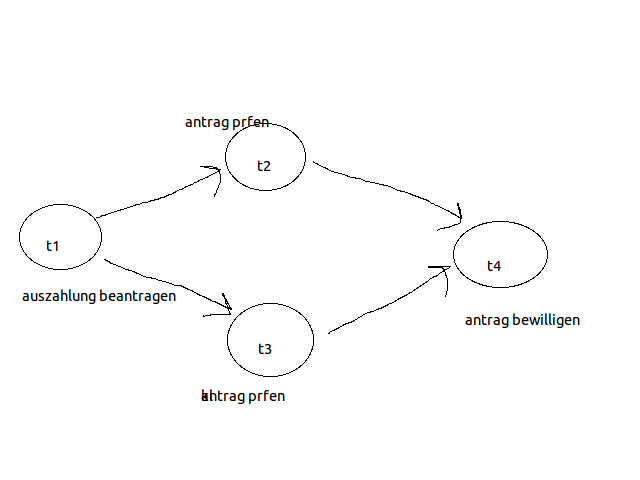
\includegraphics[width=0.9\textwidth]{Figures/Workflow}
	\caption{Arbeitsablauf in einer Bank, nachdem ein Kreditantrag eingegangen ist.}
	\label{fig:WorkflowEinleitung}
\end{figure}

Sobald ein Kreditantrag bei der Bank eingeht, muss dieser geprüft werden. Je nach Ergebnis der Prüfung, wird der Antrag entweder bewilligt oder abgelehnt. In jedem Fall muss der Kunde wieder kontaktiert werden.
Da es nicht erwünscht ist, dass der selbe Mitarbeiter, der den Antrag aufnimmt, ihn auch prüft, wird hier das \textit{Separation of Duty Prinzp} angewendet. Im einfachsten Fall würde der Prüfer die Fehler oder Falschangaben im Antrag entdecken und ihn zurückweisen. Ein schwierigeres Szenario ist, wenn sich zwei Angestellte absprechen und sich gegenseitig ihre Anträge bewilligen. Ein \textit{SOD} Modell, welches jeden Arbeitsablauf für sich betrachtet, würde diesen Betrug nicht erkennen. Es wird eine Lösung benötigt, auch Einschränkungen zwischen mehreren Instanzen eines Arbeitsablaufs zu definieren. Um den Schaden gering zu halten, könnte man verbieten, dass zwei Mitarbeiter in mehr als drei Arbeitsabläufen gemeinsam an T1 und T2 arbeiten.



%-----------------------------------
%	Ziel der Arbeit
%-----------------------------------

\section{Ziel der Arbeit}

Ziel der Arbeit ist es, eine Definitionssprache zu entwickeln, die es ermöglicht, Einschränkungen und Regeln zur Ausführung von Aufgaben durch bestimmte Angestellte sowohl innerhalb von Prozessinstanzen als auch zwischen mehreren Instanzen zu definieren. Dazu muss untersucht werden, welche Arten von Einschränkungen und Regeln es gibt und wie die Spannweite einer Regel definiert werden kann. Anschließend wird ein Modelchecker entwickelt, der \textit{Eventlogs} auf die Einhaltung dieser Regeln untersucht.



%-----------------------------------
%	AUFBAU DER ARBEIT
%-----------------------------------

\section{Aufbau der Arbeit}
Folgende Konventionen werden hier eingehalten:\\
\textit{kursive Begriffe  bezeichnen Fachbegriffe}\\
\textbf{Definitionen und Abkürzungen werden beim ersten Vorkommen fett geschrieben}\\
\texttt{Blockschrift kennzeichnet Pseudocode, Klassennamen, Code und Programmbefehle}\\

Diese Arbeit setzt ein elementares Verständnis von Logik und logischer Programmierung voraus, da hier nicht näher darauf eingegangen wird.

In Kapitel 2 wird einerseits ein Überblick über die Grundlagenliteratur gegeben als auch verwandte Arbeit vorgestellt. Dabei wird kurz darauf eingegangen, inwiefern sich diese Arbeit von den Anderen unterscheidet. In Kapitel 3 werden wichtige Begriffe erläutert. In Kapitel 4 widmen wir uns der  Herleitung von Einschränkungen und der Definition einer entsprechenden Grammatik. Diese wird in Kapitel 5 in ein Programm integriert, welches Event Logs auf die Verletzung von Einschränkungen prüft. Dazu wird der Algorithmus und der Aufbau des Programms vorgestellt. In Kapitel 6 wird ein Beispiel zur Funktionsweise des Programms präsentiert. Schließlich wird die Arbeit in Kapitel 7 noch einmal zusammengefasst.

